% !TeX spellcheck = en_US
% !TEX root = ../thesis.tex
\chapter{Background} \label{ch:background}
\section{Machine learning}
Human beings learn by experience, part of which is inherited from previous generations. However, in the digital world, experiences can be stored in form of data, which can be later processed and analyzed.

We live in the middle of a data deluge. The technological progress and the Internet have boosted our logging and communication capacities. At the time of writing this paragraph\footnote{https://www.internetlivestats.com/one-second/ on February 6th 2022.}, every single second 10,000 new tweets are written, 100,000 search queries are sent to \textit{Google}, 100,000 videos are being viewed in \textit{YouTube}, and 3,000,000 emails are sent. All amounts to approximately a 140 terabytes of Internet traffic per second.

This \textit{Brobdingnagian} amount of data cannot be analyzed without the help of automated computational assisted tools, and this is exactly the purpose of machine learning. More formally, we define machine learning as a set of computational methods designed to automatically learn hidden structures and patterns from the data and its origin \autocite{murphy2012, theodoridis2015}. Machine learning algorithms can serve multiple purposes ranging from informing decision making under uncertainty to understand and simulate natural processes. Sometimes, machine learning algorithms are inspired in biological processes \autocite{haykin1998} or in how the brain works and learns (e.g. \textit{self-organizing maps}; \citealp{kohonen2001}). Other times, machine learning is driven by specific needs arising from data analysis problems (e.g. binary decision trees; \citealp{hastie2009, hastie2014}).

\section{Types of learning}
Machine learning algorithms are designed to learn from data. However, there are many ways these data can be treated in the learning process. In this section, the most common types of learning are described at a high level.

\subsection{Supervised learning}
Supervised learning is the most widely employed methodology to train machine learning models. It is based on a function-fitting perspective, where the function $f_\theta$ is adjusted (or trained, in the machine learning jargon) to map a set of input vectors $\mathbf{X}$ to the corresponding output vectors $\mathbf{Y}$ ($f_\theta:\mathbf{X}\rightarrow \mathbf{Y}$), given a set of $N$ input pairs $\mathbf{T}=\{(\mathbf{x_i},\mathbf{y_i})\}_{i=0}^{N}$ known as the training dataset \autocite{theodoridis2015}. The learning algorithm adjusts the parameters $\mathbf{\theta}$ of a function $f_\theta$ according to the minimization of a predefined cost function $J$ (for example the mean squared error between the predicted values and the labels; \citealp{hastie2009}). The vector $\mathbf{x_i}$ (with length $D$, $\mathbf{x_i} \in \mathbb{R}^D$) represents a set of features (e.g. the age and the income of a person)  and $\mathbf{y_i}$ (with length $K$, $\mathbf{y_i}\in\mathbb{R}^K$) is the vector of response variables (representing for instance the probabilities to buy a set of products)\footnote{Notice that we represent the output $\mathbf{y_i}$ as a vector although supervised models can be univariate. However, the multivariate form is a more general case.}.

There are two main forms of supervised learning  \autocite{murphy2012}.

\begin{itemize}
	\item \textit{Regression}, where the task consists of mapping each input vector $\mathbf{x_i}$ to a real-valued vector $\mathbf{y_i} \in \mathbb{R}^K$. An example of this task would be predicting the age of an \textit{abalone}\footnote{A type of marine snail.} based on physical measurements of the different parts of its body \autocite{dua2019abalone}.
	\item \textit{Classification}, where a task consists of mapping the input vectors $\mathbf{x_i}$ to nominal variables from a finite set $\mathbf{C_j}$, with $y_{i,j} \in \{1,2,...,||\mathbf{C_j}||\}$, where $||\mathbf{C_j}||$ is the cardinality of the $j$-th response set. An example of a classification task would be determining if a mushroom is poisonous or edible based of several physical characteristics \autocite{dua2019abalone}.
\end{itemize}

\subsection{Unsupervised learning}
Unsupervised learning techniques are employed when no labeled data is available. The training dataset is composed of a set of input vectors $\mathbf{U}=\{(\mathbf{x_i})\}_{i=0}^{N}$, and the objective consists on finding interesting patterns in the data. Compared to supervised learning, unsupervised learning comprises a wider range of techniques and its objective is less well defined: the models have no clear desired output nor obvious error metric \autocite{Goodfellow2016}. However, the unsupervised learning paradigm seems to be closer to the way animals and humans learn. These algorithms also provide a cheaper framework for data exploitation, given that no data annotation is required by human experts, which is generally expensive.

Some of the most common applications of unsupervised learning are described below.

\begin{itemize}
	\item \textit{Clustering}: consists of finding dissimilar subpopulations in the data (also known as clusters or groups), where the elements within a subpopulation are more similar between them than to elements in other subpopulations.
	\item \textit{Probability density or mass estimation}: the machine learning algorithm is trained to learn the probability density function of the data (or the probability mass function in case $\mathbf{X}$ is discrete) $p_{model}(\textbf{X}): \mathbb{R}^N \rightarrow \mathbb{R}$ \autocite{Goodfellow2016}. For this, the model needs to learn the underlying structure of the data $\mathbf{X}$. The techniques laying in this family can be used for many downstream applications, such as clustering \autocite{wang2006}, missing data imputation \autocite{qichuan2015} or generation \autocite{liu2020a}.
	\item \textit{Manifold learning}: is a set of techniques consisting of learning the structure of high-dimensional data, where the data is assumed to lie on a low-dimensional manifold in a high-dimensional space \autocite{murphy2012}. The objective of these techniques is to discover latent structures in the data that can be exploited for tasks such as data compression, dimensionality reduction, feature extraction or data visualization. One example of this task could be reducing the dimensionality of a dataset using \textit{principal components analysis} (PCA). That would project the original dataset linearly into a lower dimensional one with orthogonal axes, where the structures in the data could presumably be more easily discernible.
	\item \textit{Data completion}: consists of imputing the missing values of a given dataset \autocite{vanburen_2018}. This can be done with different purposes such as inferring the unfilled optional answers of a survey, or filling the gaps of a time series with low sampling frequency to get a higher time resolution representation. Some forms of collaborative filtering \autocite{falk2019}, for example matrix factorization algorithms \autocite{koren2009}, can also be seen as a data completion task where the algorithm needs to fill the blanks of a matrix representing the ratings of products by customers. In these cases, the algorithm needs to answer a question similar to: what would be the rating that a given customer would assign to a given product if they had the chance?
	\item \textit{Associative learning}:  is a type of unsupervised learning where the goal is to discover the relationships between objects in the data \autocite{zhang2002}. These relationships can be expressed in terms of associations (e.g. if A then B), correlations (e.g. A is positively correlated with B) or co-occurrence (e.g. A and B are often observed together). One example of associative learning would be applying the \textit{Apriori} algorithm \autocite{agrawal1996} to a supermarket database in order to discover the most interesting associations between different products with the aim of deriving attractive offers for customers, or optimize product placement to improve customer experience. 
	\item \textit{Generative modeling}: many forms of generative model also rely on unsupervised learning techniques \autocite{bishop2006}. This task consists on learning to approximate $p(\mathbf{X})$ with the objective of generating data that is indistinguishable from the original distribution. It is often done by maximizing the likelihood of the data given the model $\mathrm{argmax}_\mathbf{\theta} p(\mathbf{\mathbf{X},\mathbf{\theta}})$. However, in cases where the explicit density function is not needed, other methods may apply (this topic will be covered more in depth in section \ref{sec:generative}).  One example of application of these techniques would be in the field of natural language processing, where the goal is to learn a model that can generate text \autocite{uday2019} that is realistic and linguistically plausible (these are commonly known as language models).
\end{itemize}


\subsection{Reinforcement learning}
Reinforcement learning is a family of machine learning algorithms which, in contrast to the other types of learning, does not necessarily rely on any previously gathered knowledge about the task at hand. Instead, the reinforcement learning agents (or decision makers) learn what to do by mapping situations to actions \autocite{sutton2018} so that they maximize a numerical reward metric, usually in presence of uncertainty \autocite{haykin1998}. For the agent to learn successful behaviors (referred commonly as policies), it needs to balance exploration and exploitation while interacting with the environment \autocite{sutton2018}, in simpler terms, reinforcement learning algorithms learn by trial and error.

More formally, the environment is commonly formulated as \textit{finite-discrete-time Markov decision process} \autocite{haykin1998}, which can be represented as a 4-tuple: ($S$, $A$, $P_a$, $R_a$) where $S$ represents the state space, $A$ is the action space, $P_a(s, s')$ is the probability of transitioning from state $s$ to state $s'$ after performing the action $a$, and $R(s, s', a)$ is the reward received when transitioning from state $s$ to state $s'$ after performing action $a$. 

The objective of the learning algorithm is to build an agent such that its policy $\pi_\theta(s)$ maximizes the expected sum of discounted rewards $\mathbb{E} \left[ \sum_{t=0}^{T} \gamma^t R(s_t, s_{t+1}, a) \right]$, where $\gamma$ is usually a scalar number between 0 and 1. The reinforcement learning theory is originally based upon dynamic programming \autocite{szepesvari2010}.

A classical example of a successful reinforcement learning application can be found in \autocite{tesauro1994}, where an agent is trained to play \textit{Backgammon} game.

Detail treatment of the reinforcement learning field lies far beyond the scope of this thesis. A more detailed introduction is given in \autocite{sutton2018, szepesvari2010}.

\subsection{Other types of learning} \label{sec:typesoflearning_others}
There are other learning paradigms \autocite{raghu2020} that are worth mentioning, but either it is not clear where they lay, or they combine elements from various of the previously discussed types of learning. The following list describes the most important ones.
\begin{itemize}
	\item \textit{Semi-supervised learning algorithms} learn from both labeled and unlabeled data. This is beneficial in problems where it is difficult or costly to label the data, and hence the amount of labeled data is scarce \autocite{raghu2020}. One example of field where semi-supervised learning has many potential applications is fraud detection \autocite{wang2020b}, where these cases are uncommon by nature and difficult to spot.
	\item \textit{Self-supervised learning algorithms} aim to solve what is known as a \textit{pretext task}: a supervised problem where the data can be automatically labeled without human intervention, without extra cost and directly from the raw instances \autocite{raghu2020}. One example of \textit{pretext task} could be determining the missing word in a partially masked sentence, given a set of sentences extracted from a collection of books \autocite{devlin2019}, with the aim of learning latent representations of the words. Other example could be determining the degree of rotation of an image \autocite{gidaris2018} for biasing the model towards learning the latent structure of the images.
	\item \textit{Transfer learning} is a discipline solely applicable to deep learning models. This methodology consists of two steps: pre-training a model to solve a large and generic task (e.g. classify large and full-color images into 1000 categories \autocite{deng2009imagenet}) and then fine-tuning the pre-trained model to solve a different target task \autocite{raghu2020}. This paradigm has a lot of benefits in multiple applications (for instance when restricted amounts of labeled data are available, or when the computational resources available are limited). As an example, the authors of \autocite{souza2022} show how they got successful results in performing sentiment analyses over user reviews by using pre-trained word embeddings based on \textit{BERT} \autocite{devlin2019}. Further details about transfer learning will be covered in the chapter \ref{ch:distillation} of this thesis.
\end{itemize}


\section{Deep learning}

Deep learning algorithms were motivated by the failure of classical machine learning algorithms on solving central problems on AI (e.g. speech recognition, object recognition, text generation, etc). These algorithms have a long history (figure \ref{fig:dl-timeline} summarizes the most important events in the development process of deep learning), and have been named differently along the years: connectionist models, artificial neural networks, deep learning, etc.

\begin{figure}
	\centering
	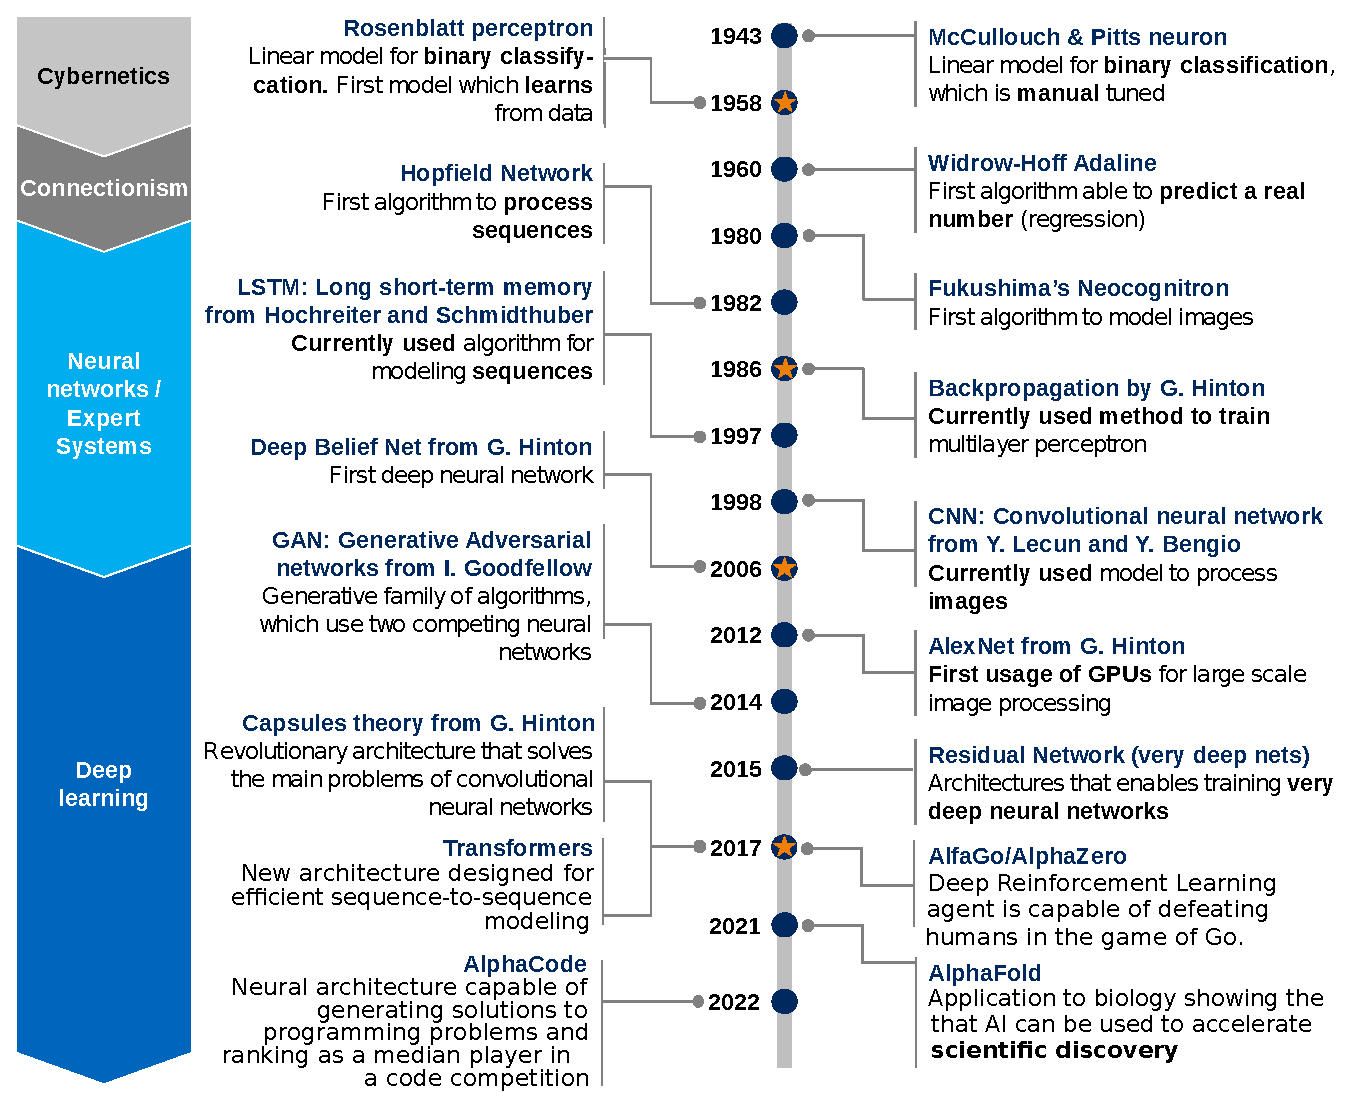
\includegraphics[width=1.0\linewidth]{background/images/DL-timeline}
	\caption[Deep learning history timeline]{Timeline showing the most important achievements in the research of what is currently known as deep learning.}
	\label{fig:dl-timeline}
\end{figure}


Deep learning is a subfield of artificial intelligence and machine learning as shown in the \textit{Venn} diagram of figure \ref{fig:venndl} (reproduced from \cite{Goodfellow2016}), and provides a very flexible framework for different machine learning tasks, spanning all the aforementioned types: supervised, unsupervised, reinforcement learning and others.

\begin{figure}
	\centering
	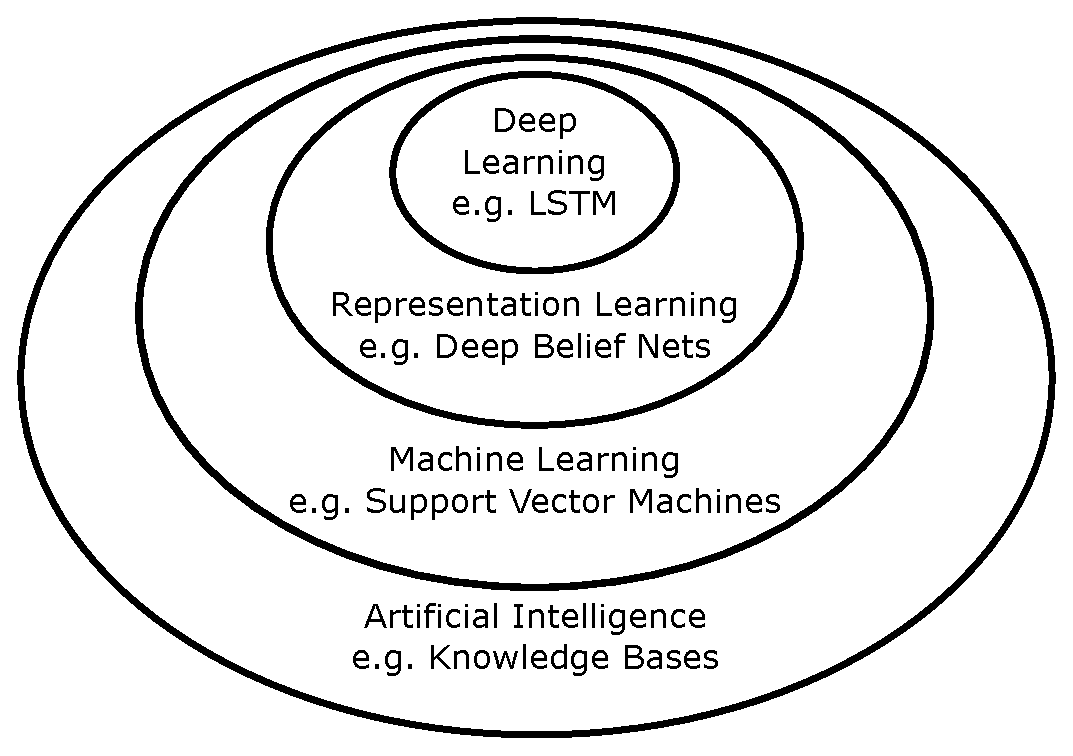
\includegraphics[width=0.5\linewidth]{background/images/venn_DL}
	\caption[Deep learning \textit{Venn} diagram]{Deep learning context within the artificial intelligence field \autocite{Goodfellow2016}}
	\label{fig:venndl}
\end{figure}



\subsection{From the perceptron to its multilayer version} \label{sec:mlp}

This section introduces the basic feed-forward neural network, from its origin to the modern trends. The basic component of a modern deep learning model is the artificial neuron (sometimes called unit). The idea of an artificial neuron has its origin in the \textit{McCulloch-Pitts} model from 1943, an attempt to mathematically model the functionality of a biological neuron \autocite{mccullochPitts1943}. The \textit{McCulloch-Pitts} neuron consisted of a linear function of a set of binary inputs $\mathbf{x}$ that are multiplied by a set of weights $\mathbf{w}$ (which values are either excitatory or inhibitory, i.e. 1 or -1), the result is added together, a threshold scalar is subtracted to the result, and a sign function is applied to produce a binary output $y$ (see figure \ref{fig:mcpittsneuron} for a graphical description). The whole model is described in equation \ref{eq:mcpitts}. This weights and the threshold were meant to be adjusted manually by an operator.

\begin{figure}
	\centering
	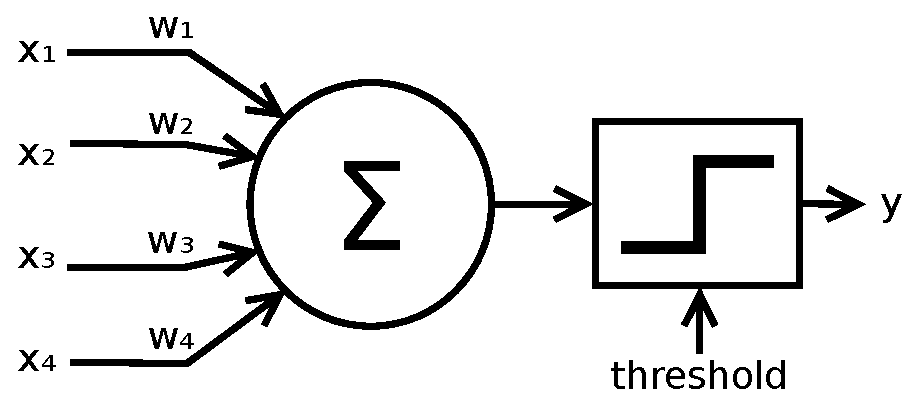
\includegraphics[width=0.60\linewidth]{background/images/mcpittsneuron}
	\caption[\textit{McCulloch-Pitts} neuron model]{\textit{McCulloch-Pitts} neuron model, with 4 input variables $\{x_i\}$ and one output $y$. $\{w_i\}$ represent the synaptic weights of the neuron.}
	\label{fig:mcpittsneuron}
\end{figure}

\begin{equation}
	\label{eq:mcpitts}
	y_i = \mathrm{sgn}\left(\sum_{j=1}^{D} x_{i,j} \cdot w_{j} - \mathrm{threshold}\right)
\end{equation}

Some years later, \textit{Frank Rosenblatt} introduced the \textit{perceptron} \autocite{Rosenblatt58}. His idea builds upon the \textit{McCulloch-Pitts} model, proposing a simple method to automatically learn the weights of the model (see equation \ref{eq:rosenblatt}, where the desired response is represented by $y_j$, the predicted one is represented by $\hat{y}_j$ and $\lambda$ is a scalar that controls the size of the weight updates, commonly referred as the learning rate). This is considered the first primitive neural network.

\begin{equation}
\label{eq:rosenblatt}
\mathbf{w_j(t+1)} = \mathbf{w_j(t)} + \lambda [ y_j-\hat{y}_j(t) ] \cdot \mathbf{x_j}
\end{equation}

 A couple of years later, \textit{Bernard Widrow} and his student \textit{Ted Hoff} proposed the \textit{ADALINE} model (ADAptive LINear Element) \autocite{widrow1960}, a modification of the \textit{McCulloch-Pitts} model that removed the sign function. \textit{ADALINE} was trained using gradient descent \autocite{fredric2000}, as described in equations \ref{eq:adaline_gd} and \ref{eq:adaline_step}, where $\lambda$ is the learning rate and $N$ is the number of training examples (these equations are commonly known as \textit{the delta rule}).
\begin{equation}
\label{eq:adaline_fp}
y_i = \sum_{j=1}^{D} x_{i,j} \cdot w_{j} + b
\end{equation}

\begin{equation}
\label{eq:adaline_gd}
\frac{\partial J}{\partial{w_j}} = \frac{1}{N} \sum_{i=1}^{N} x_{i,j} \cdot(\hat{y}_i - y_i)
\end{equation}

\begin{equation}
\label{eq:adaline_step}
\mathbf{w_j(t+1)} = \mathbf{w_j(t)} - \lambda \cdot \frac{\partial J}{\partial {w_j}}
\end{equation}


 The combination of multiple \textit{ADALINE}-style perceptrons with activation functions such as the sigmoid function (see equation \ref{eq:mlp}, where $g$ represents a non-linear activation function), builds a \textit{multilayer perceptron} (\textit{MLP}). More specifically, a \textit{MLP}, also known as \textit{fully-connected} neural network, is a neural architecture whose building blocks are perceptrons (called neurons in this scenario) which are disposed in layers so that all the elements from a layer $l$ are connected with all the elements in the next layer $l+1$ (refer to figure \ref{fig:mlp} for a visual example)


 \begin{equation}
 \label{eq:mlp}
 h_i = g\left(\sum_{j=0}^{D} x_{i,j} \cdot w_{j} + b\right)
 \end{equation}

 The \textit{delta rule}, described in equations \ref{eq:adaline_fp} and \ref{eq:adaline_gd}, built the basis for the \textit{backpropagation} algorithm, a methodology widely used nowadays as standard method to train neural networks. The \textit{backpropagation} algorithm \autocite{hinton1986} was published by \textit{David Rumelhart} and \textit{Geoffrey Hinton} in 1986 as a method to optimize the parameters of \textit{multilayer perceptrons}. This algorithm comprises two steps \autocite{haykin1998}:

\begin{enumerate}
\item \textit{Forward pass}: consisting on a simple model inference operation, where a set of features $\mathbf{x}_i$ are fed to the network as input to get the output $\mathbf{\hat{y}_i}$. In this phase, some of the values of the intermediate neurons can be cached to use them in the next step.

\item \textit{Backward pass}: a metric $J$ (often referred as cost or loss function) is used to compare the outputs of the model $\mathbf{\hat{y}_i}$ with the desired outputs (sometimes called targets) $\mathbf{y_i}$ and then propagate the gradient of the error backwards (from the output to the input), by using the chain rule, to adjust the weights of the model.
\end{enumerate}


\begin{figure}
	\centering
	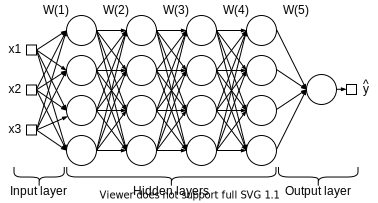
\includegraphics[width=0.8\linewidth]{background/images/mlp}
	\caption[Multilayer perceptron]{Example of \textit{multilayer perceptron} with 3 inputs, 1 output and 3 hidden layers. Each bubble represents a neuron (figure \ref{fig:mcpittsneuron}), and has an associated bias term. Each arc represents a weight. In each neuron, the inputs multiplied by their corresponding weights are added to the neuron's bias, and then an activation function is applied to produce the output, according to equation \ref{eq:mlp}.}
	\label{fig:mlp}
\end{figure}


Before \textit{backpropagation}, there was no algorithm for training \textit{multilayer perceptrons} in an end-to-end manner. The only way to train those models was to fix the weights of all but one layer, and train the free one with gradient descent or other methods. These models were called feature analyzers \autocite{hinton1986}, and one of the most interesting examples is the \textit{Gamba} perceptrons, described in \citet{minsky69}. Although it is out of the scope of this thesis, it may be worth mentioning that modern versions of the \textit{Gamba perceptron} (known as \textit{Extreme Learning Machines}) are still in the research community spectrum as alternative training methods to \textit{backpropagation} see \autocite{Huang2006, Huang2012}.

The introduction of \textit{backpropagation} enabled the neural networks to learn their own hidden representations automatically, allowing for more complex and abstract models. One of the most important pieces of \textit{multilayer perceptrons} and other modern architectures are the neuron \textit{activation functions} (also referred sometimes as \textit{nonlinearities}). An \textit{ADALINE} style neuron is a linear function, and linear functions are closed under composition, therefore the composition of several \textit{ADALINE} neurons is a linear function. To break the linearity of the neurons, the \textit{activation functions} are introduced. They consist of non-linear functions which are applied to the output of each neuron. The authors of \autocite{hinton1986} formulated the \textit{backpropagation} algorithm with sigmoid activation functions (defined in equation \ref{eq:sigmoid}), as a differentiable alternative to the classical sign function. Later, it was discovered that unbounded and non-smooth \textit{nonlinearities} like the \textit{Rectified Linear Unit} (\textit{ReLU}; \citealp{nair2010}; defined in equation \ref{eq:relu}) were more convenient for training deep architectures \autocite{Goodfellow2016}. Activation functions are discussed in depth in chapter \ref{ch:modulus}.


\begin{equation}
\label{eq:sigmoid}
f(x) = \frac{1}{1+e^{-x}}
\end{equation}

\begin{equation}
\label{eq:relu}
f(x) = \max(x, 0) =
\begin{cases}
x,          & \text{if } x \geq 0 ,\\
0,         & \text{otherwise},
\end{cases}
\end{equation}

The \textit{backpropagation} algorithm has certain rules that need to be met \autocite{hinton1986}: (1) connections from higher level neurons to lower level ones are forbidden, but connections that skip layers are totally permitted, (2) the architecture must be fully differentiable to be able to backpropagate the errors, and (3) the weights must not all be initialized to the same fixed value, but they must be set to random values instead, to break the symmetrical weights between layers (which would cause the optimization to stall, see \autocite{hinton1986} for more details). 


Despite meeting these rules, there are no theoretical guarantees for the algorithm to find the global minimum: it can get stuck in local minima. One possible way to avoid this problem consists of running the optimization several times with different random parameter initializations \autocite{haykin1998}. The usage of gradient-free methods such as evolutionary optimization techniques \autocite{sivanandam2008} have also been explored by the deep learning research community, sometimes leading to promising results \autocite{omid2014, vallesperez2012}. However, these algorithms are usually less computationally efficient than gradient-based ones, making them unfeasible when the training data or the model size are large.

\subsection{Neural networks as universal approximators}
Given any continuous function $f(x)$ with arbitrary complexity, it is always possible to find a multilayer perceptron with a single hidden layer and sigmoid activations that approximates that function to any desired degree of accuracy.

This problem was originally formulated and solved by \citealp{Cybenko1989}. In particular, the work proves that:

\begin{thm}[2 - Cybenko, 1989]
	Let $\sigma$ be any continuous sigmoidal function. Then finite sums of the form

	$$ G(x) = \sum_{j=1}^{N} \alpha_j \sigma(w_j^Tx + \theta_j) $$

	are dense in $C(I_n)$. In other words, given any $f \in C(I_n)$ and $\epsilon > 0$, there is a sum, $G(x)$, of the above form for which

	$$|G(x) - f(x)| < \epsilon \quad \forall x \in I_n$$
\end{thm}

For the sake of gaining intuition (refer to \citealp{Cybenko1989} for a formal proof), let $G$ be a \textit{multilayer perceptron} with a single hidden layer, whose neurons have a sigmoid activation. Assuming the weights of the hidden layer are set to a sufficiently large number, it can be easily seen that the sigmoid activations approximate a \textit{Heaviside step function} $H$ (see equation \ref{eq:sigmoidToHeaviside}, where $\delta$ represents a very large number). Then, by adding infinitely many \textit{Heaviside} functions with the proper shift and scaling, one can easily approximate any continuous function. It can also be seen that the shift and scaling operations correspond to the bias of the neurons in the hidden layer and the weights of the output layer, respectively.

As it can be seen in figure \ref{fig:universalapprox}, by increasing the number of neurons one can easily control the fidelity of the approximation. This theorem proves that if we have arbitrarily many neurons in the hidden layer, a \textit{multilayer perceptron} with only one hidden layer can approximate any continuous function to an arbitrary degree of precision.


\begin{figure}[h!]
	\centering
	\includegraphics[width=1\linewidth]{background/images/universalapprox}
	\caption[Universal approximation theorem visual example]{In the left side, a toy \textit{multilayer perceptron} with a single hidden layer, a single input and a single output, and with the weights of the hidden layer set to a very large number $\delta$. The bias terms have been indicated inside the bubbles. In the right hand side, a target function $f(x)$ to be approximated (smooth dashed blue line) and the approximation $G(x)$ (thick solid line) achieved given the weights and biases in the network of the left. The different segments of the approximation have been colored with the same color as the last neuron that fired to set that value, as the value of $x$ increases.}
	\label{fig:universalapprox}
\end{figure}

\begin{equation}
	\label{eq:sigmoidToHeavyside}
	\lim_{\delta \rightarrow \infty} (\sigma(\delta x)) = \mathrm{H}(x)
\end{equation}



After \textit{Cybenko}, other studies \autocite{Leshno1993, pinkus1999} proved that the theorem holds for non-sigmoid activation functions as well. Despite the universal approximation theorem (theorem 1) proving that a single hidden layer is enough to model any arbitrarily elaborated continuous function, deeper neural networks are motivated by the fact that more sophisticated functions may approximate complex problems more easily and efficiently, perhaps even needing less parameters \autocite{nguyen21}.



\subsection{Deeper neural networks} \label{sec:deepernn}
Regardless the emergence of the \textit{backpropagation} algorithm, training a \textit{multilayer perceptron} with many layers was \textit{challenging}. The first successful methodology for training deep neural networks consisted on pre-training the weights of the network in an unsupervised fashion, using stacks of \textit{restricted Boltzmann machines} (RBM; \citealp{Smolensky1986}) known as deep belief networks \autocite{hinton2006, Bengio2007}. A \textit{restricted Boltzmann machine} (initially called \textit{Harmonium}) is a type of neural network built using a bidirectional bipartite graph architecture, with symmetric connections of neurons between the two layers and without connections between neurons within the same layer (as shown in figure \ref{fig:rbm}). This model is trained to learn hidden abstract representations of the input, from which it is possible to recover the original probability distribution $p_\theta(x|h) \approx p(x)$. The training procedure is based on an approximate \textit{maximum-likelihood} method called \textit{contrastive divergence} (CD; \citealp{hinton2002}).

\begin{figure}[h!]
	\centering
	\includegraphics[width=0.3\linewidth]{background/images/rbm}
	\caption[\textit{Restricted Boltzmann machine}]{\textit{Restricted Boltzmann machine} with 5 visible units and 3 hidden units.}
	\label{fig:rbm}
\end{figure}

Deep belief networks are stacks of RBMs that are trained using a greedy layer-wise strategy, in which the output of a trained RBM becomes the input of the following RBM \autocite{hinton2006} (see figure \ref{fig:dbn}). It was shown in \autocite{Bengio2007} that, by following this procedure and then fine-tuning the weights of the full network using the backpropagation algorithm, deeper networks could be trained.


At the time of writing this thesis, unsupervised pre-training methods are no longer needed to train deep neural networks. This is thanks to a set of techniques that have been recently developed (in the 21st century) and that, when combined together, facilitate the convergence of the \textit{backpropagation} algorithm when used to optimize deep architectures. The first technique was the \textit{ReLU} \autocite{nair2010} activation functions (see equation \ref{eq:relu}), a non-saturating alternative to the classical functions like \textit{sigmoid} (see equation \ref{eq:sigmoid}) or $\mathrm{tanh}$, that showed to be effective at favoring sparse connectivity, and helped overcome the saturating gradients problem, a well known failure mode of neural architectures with saturating \textit{nonlinearities} when trained by \textit{backpropagation} \autocite{Hong2019}. Another simple technique that helped training deep neural networks is known as \textit{Dropout}, a regularization technique that consists of randomly zeroing out a fraction $p$ of neurons from each layer in each training step \autocite{hinton2012, srivastava2014}. These two techniques (among others) allowed \citealp{krizhevsky2012} to successfully train \textit{AlexNet}  without unsupervised layer-wise pre-training, a deep neural network that won the \textit{ImageNet} \autocite{deng2009imagenet} computer vision contest in 2012, a problem consisting of classifying millions of images into 1,000 categories. These techniques are still used today in the majority of the deep learning models that are published.

\begin{figure}
	\centering
	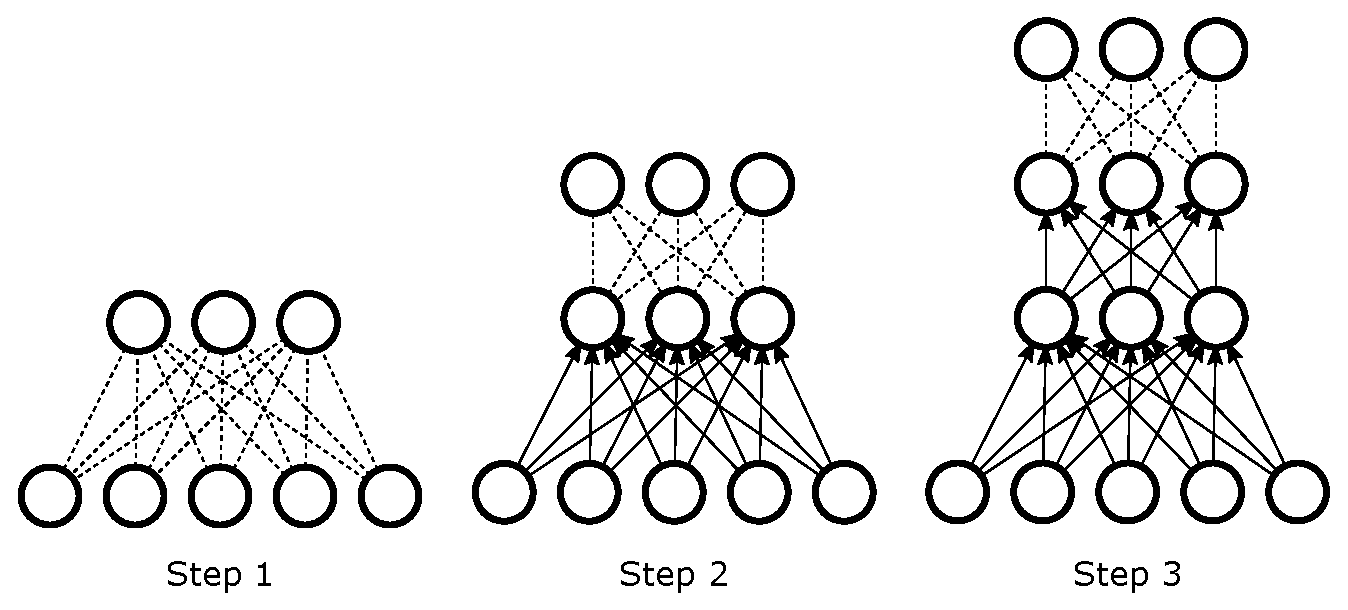
\includegraphics[width=1\linewidth]{background/images/dbn}
	\caption[Deep belief network]{Example of \textit{deep belief network} architecture with three feature detector layers. In each of the steps shown above, the dashed connections between units represent the \textit{RBM} being trained, while the solid connections represent the previously trained \textit{RBMs} that are used to compute the input of the next \textit{RBM}.}
	\label{fig:dbn}
\end{figure}



Other tricks that are commonly used nowadays to facilitate the parameters optimization of deep architectures are batch normalization \autocite{ioffe2015} and residual learning \autocite{kaiming2016}. 
\begin{itemize}
	\item \textit{Batch normalization} consists of standardizing the output vectors from hidden layers using the first and the second statistical moments (mean and variance) of the current mini-batch \autocite{ioffe2015}. This method has proved to increase the training stability when high learning rates ($\lambda$) are used \autocite{Goodfellow2016}. Additionally, it has been shown that it provides regularization \autocite{dauphin2021} as a side effect, due to the random fluctuations in the statistical moments from one batch to another.
	\item \textit{Residual learning} consists of adding skip connections between layers of the neural network, so that the output of one layer $l$ is fed as input to layer $m > l+1$. Figure \ref{fig:residual} shows an example of a graph with a residual block skipping two layers. More formally, the output of the residual block becomes $\mathbf{H(x)} = \mathbf{F(x)} + \mathbf{x}$ where $\mathbf{F(x)}$ is the function learned by the composition of the two layers and the \textit{ReLU} function\footnote{Notation disambiguation: $H(x)$ here does not refer to the \textit{Heaviside} function.}. Obviously one can see that $\mathbf{F(x)}$ is learning a residual mapping $\mathbf{F(x)} = \mathbf{H(x)} - \mathbf{x}$ \autocite{kaiming2016}. This method has empirically shown substantial improvements of the \textit{backpropagation} optimization process given that the residual connections allow gradients to flow more easily, avoiding vanishing gradients \autocite{Goodfellow2016}. \citealp{kaiming2016} were able to get the first place in the 2015 \textit{ImageNet} contest, improving the performance of \textit{AlexNet}. Recent studies found that residual connections help reform the loss landscape leading to more convex optimization surfaces \autocite{freeman2017, wang2020a}.
\end{itemize}
 


\begin{figure}[h!]
	\centering
	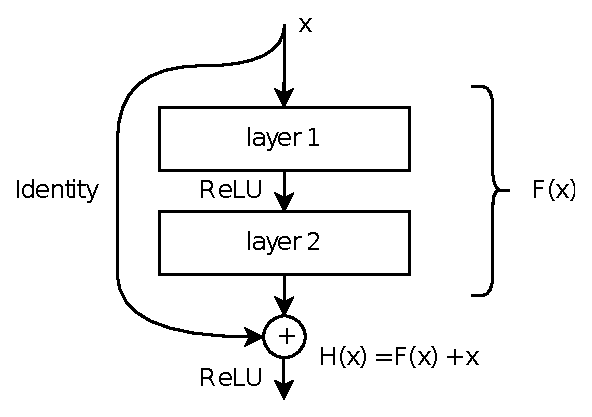
\includegraphics[width=0.5\linewidth]{background/images/residual}
	\caption[Example of a residual block]{Example of a residual block.}
	\label{fig:residual}
\end{figure}


Finally, another difference between modern and classical deep learning models is the extended use of \textit{mini-batch} stochastic gradient descent (see equation \ref{eq:mbsgd}), where successive optimizations steps are performed by \textit{backpropagation} using small ($m$-sized) random subsamples of the dataset named \textit{mini-batches} \autocite{ruder2016}. Previous alternatives were stochastic gradient descent, where the updates are performed for every individual sample, and batch gradient descent, where the updates are performed over the full dataset $\mathbf{T}$. \textit{Mini-batch} gradient descent has shown generalization improvements over the batch method \autocite{Hoffer2017}, while being computationally more efficient than the \textit{stochastic gradient descent} method.


\begin{equation}
	\label{eq:bgd}
	\mathbf{\theta}(t+1) = \mathbf{\theta}(t) - \lambda \cdot \nabla_\mathbf{\theta} J(X, Y|\mathbf{\theta}(t))
\end{equation}

\begin{equation}
	\label{eq:sgd}
	\mathbf{\theta(t+1)} = \mathbf{\theta}(t) - \lambda \cdot \nabla_\mathbf{\theta} J(x_i, y_i|\mathbf{\theta}(t)) \quad \mathrm \quad \mathrm{where} \quad (\mathbf{x_i}, \mathbf{y_i}) \sim \mathbf{T}
\end{equation}

\begin{equation}
	\label{eq:mbsgd}
	\mathbf{\theta}(t+1) = \mathbf{\theta}(t) - \lambda \cdot \nabla_\mathbf{\theta} J(x_{i:i+m}, y_{i:i+m}|\mathbf{\theta}(t)) \  \mathrm{where} \quad  (\mathbf{x_{i:i+m}}, \mathbf{y_{i:i+m}}) \sim \mathbf{T}
\end{equation}


\subsection{Modern architectures}
In this subsection, three modern building blocks frequently used in the current deep learning architectures are described from a general perspective: convolutional neural networks (CNN), recurrent neural networks (RNN) and transformers. These architectures are the backbone of the majority of deep learning applications and the computational core of the systems presented throughout the next chapters.

\subsubsection{Convolutional neural networks}
A CNN is a type of feed-forward neural network that is commonly used in problems where the input data have grid-like topology \autocite{Goodfellow2016}. Common examples of these data are time-series (1D), images (2D) or videos (3D). CNNs are not new, and one of the most important primitive CNN is known as \textit{neocognitron}, a neural architecture published by \citealp{fukushima1980}, as a model inspired in the primary cortex of the human brain that was able to recognize Japanese handwritten characters \autocite{fukushima1980}. This model was similar to modern convolutional neural networks, and even featured similar properties like weight sharing and translation equivariance (these properties are discussed below). The \textit{neocognitron} inspired future works like \textit{LeNet-5}, a 7-layer convolutional neural network (see figure \ref{fig:lenet5}) trained with \textit{backpropagation} to recognize handwritten digits \autocite{lecun1998}.

\begin{figure}
	\centering
	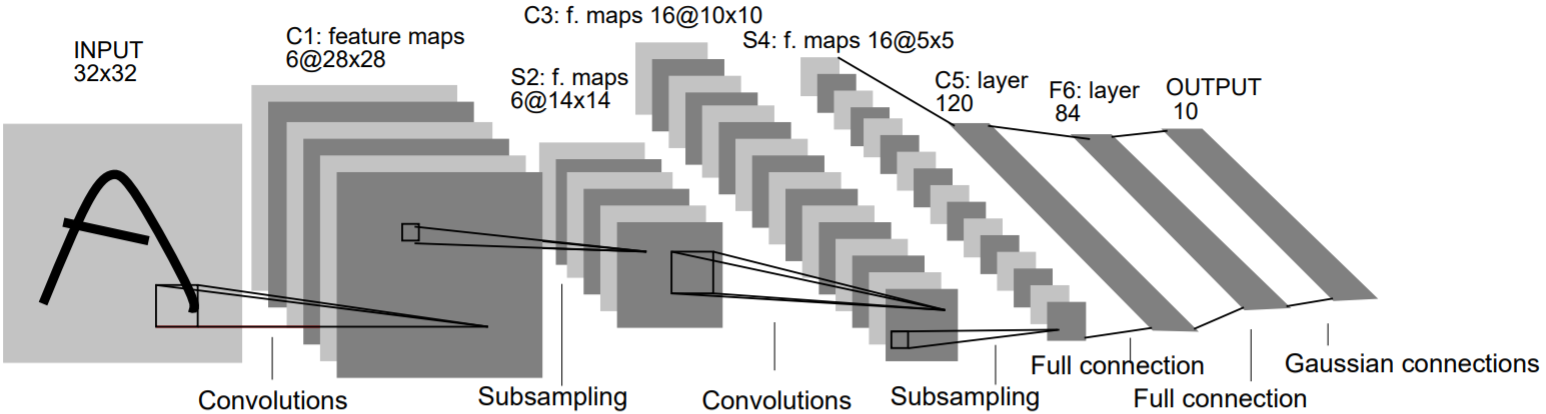
\includegraphics[width=0.85\linewidth]{background/images/lenet5}
	\caption[\textit{LeNet-5} architecture]{\textit{LeNet-5} neural architecture, with 7 layers, capable of recognizing handwritten digits.}
	\label{fig:lenet5}
\end{figure}

CNNs use cross-correlation operations\footnote{Formally, the operation is called cross-correlation. Nevertheless they are more commonly referred as convolutions by the machine learning community. In this dissertation we use both terms indistinguishably to refer to the convolutional layers operations.} instead of the general matrix multiplication used in fully connected networks. In this context, a convolution is a linear operation where an input $\mathbf{X}$ is correlated with a \textit{kernel} $\mathbf{W}$ to produce a \textit{feature map} $\mathbf{S}$ (see equation \ref{eq:cnnformula}, where $g$ represents the \textit{nonlinearity}). The task of the algorithm is to learn the \textit{kernel} to solve the target task \autocite{haykin1998}. In other words, equation \ref{eq:cnnformula} describes how the \textit{kernel} is displaced over the input image $\mathbf{X}$ to determine its similarity with the different regions of the full-color image.

\begin{equation}
	\label{eq:cnnformula}
	S_{i,j.k} = g\left(\sum_{l,m,n}{X_{i+l, j+m, k+n} \cdot W_{l,m,n} + b}\right)
\end{equation}

Convolutional neural networks are composed (sometimes partially) of convolutional layers (where several convolutional \textit{kernels} are applied in parallel). These layers have several properties that differenciate them from the classical dense layers, and that become advantageous when the input data can be arranged into a grid structure. These properties are discussed below \autocite{Goodfellow2016}.


\begin{itemize}
	\item \textit{Sparse interactions}: the units in a convolutional network are connected to a small region of neighboring inputs. The size of that region is commonly referred as \textit{receptive field}. This property drastically reduces the amount of parameters of the neural network, and enables parameters sharing.
	\item \textit{Parameter sharing}: consists of using the same parameters for more than one function in the model. This is also known as \textit{tied weights}. In a CNN, each member of the kernel is used at each position in the input (except in the special case of the boundaries, depending on the setting).
	\item \textit{Equivariance to translation}: the convolution operation builds a map representing the positions where a certain feature appears in the input (e.g. a vertical border in the case of an image). If the feature is moved in the input, its representation will be moved the same amount in the output representation. Notice that the convolution operation is not equivariant to other transformations such as rotation and scaling. This lack of properties inspired the development of the \textit{capsule networks} \autocite{sabour2017}.
\end{itemize}

Apart from the convolutions, there is another operation that is commonly used in CNNs known as subsampling. Its goal is to reduce the size of the feature maps as more layers are added, so that the representations become more generic. This helps achieve approximate invariance to translation. There are two main versions of this operation: pooling or strided convolutions. The pooling operation \autocite{Goodfellow2016} consists of computing a reducing statistic (e.g. the $\max$ function in max-pooling) over small neighboring regions. The strided convolutions \autocite{riadh2020} are standard convolutions that skip some of the inputs.

In some CNN architectures, a couple of fully-connected layers are added on top of the convolutional layers. Although, recent advances in the field have found that this is not necessary \autocite{shelhamer2015}, this pattern is commonly seen in modern architectures.

% TODO: Add modern CNN graph (maybe)

\subsubsection{Recurrent neural networks}
\sloppy RNNs are one type of neural networks that are designed to process sequential data such as time-series: $x^{(1)}, x^{(2)}, ..., x^{(T)}$, where $T$ represents the time series length. One of the most important primitive version of RNNs is known as the \citet{hopfield1982} network and was published in 1982. This network incorporated a memory cell that allowed it to process sequential data. However, it was initially designed to work with binary data.

Inspired by the \textit{Hopfield} network and its variants, the current RNNs are also incorporate memory cells (sometimes referred as the RNN internal state) that allow them to process variable-length sequences such as text sentences or audio clips \autocite{haykin1998}.

A RNN shares its weights across several time steps. This may sound similar to 1-dimensional CNNs (1D-CNNs), but there is one important difference \autocite{Goodfellow2016}: in a 1D-CNN layer, each of the elements of the output sequence is function of a small number of neighboring elements in the input sequence, whereas in the basic RNNs each element in the output is function of all the previous elements in the sequence; in other words, RNNs are causal. 

A recurrent neural network takes one input each time step, and then passed to a hidden layer that produces an output. See equation \ref{eq:RNN} for a basic example of recurrent neural network ($\mathbf{U}$ and $\mathbf{W}$ represent the trainable weight matrices, $\mathbf{b}$ is a trainable bias vector, and $\mathbf{h}$ represents the hidden intermediate representation). These hidden representations are designed to retain the important information of the previous sequence steps in order to solve the required task.

\begin{equation}
\label{eq:RNN}
\mathbf{h^{( t )}} = \mathbf{g(U h^{( t-1 )}} + \mathbf{W x^{( t )}} + \mathbf{b})
\end{equation}

The most commonly used type of recurrent neural network nowadays is the \textit{long short term memory} (LSTM). LSTMs were published by  \textit{Hochreiter} and \textit{Schmidhuber} \autocite{Schmidhuber1997} in an attempt to solve the issues of RNNs when dealing with sequences in problems that required long-term dependencies. LSTM models contain two hidden state representations: one intended to retain long term memory and other for short term memory. The architecture of a LSTM cell is composed of three gates: input gate $\mathbf{i_t}$, output gate $\mathbf{o_t}$, forget gate $\mathbf{f_t}$. These gates control how the information flows through the network, allowing to write, output and delete the states as needed. This is made possible due to the sigmoid functions, which act as valves for the different operations. Figure \ref{fig:lstm} and equations \ref{eq:LSTM} describe the LSTM cell more formally. In the equations, the symbol ``$\odot$'' refers to the \textit{Hadamard} product, $\mathbf{U}$ and $\mathbf{W}$ are trainable weight matrices, and $\mathbf{b}$ are the biases.

\begin{figure}
	\centering
	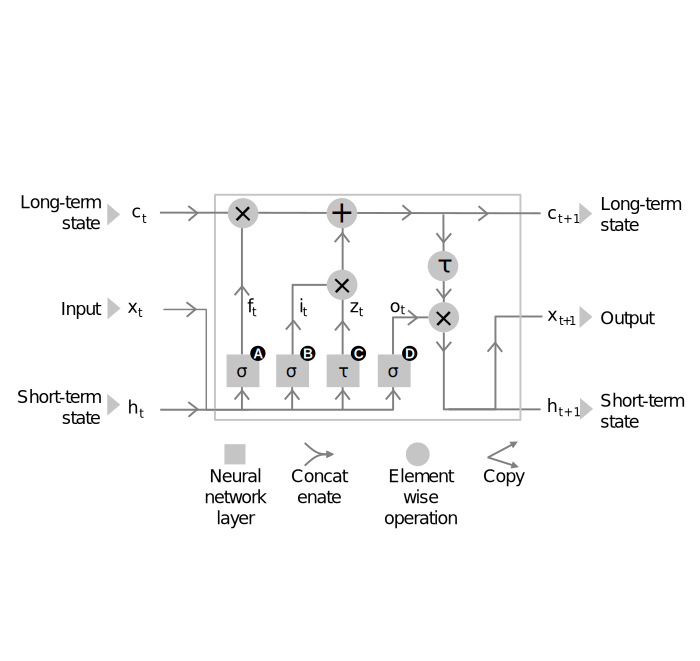
\includegraphics[width=0.7\linewidth]{background/images/LSTM}
	\caption[LSTM cell structure]{LSTM cell structure. $\mathbf{c_t}$ and $\mathbf{h_t}$ represent the long-term and short-term states, respectively, that the network uses as memory. Its operation is based on 3 gates and an output unit. (A) is a layer that acts as forget gate, represented as $\mathbf{f_t}$, which is responsible for erasing memory which will no longer be used. The layer (B) is the input gate, represented as $\mathbf{i_t}$, and controls how much input goes through the long-term line. The layer (C), represented by $\mathbf{z_t}$, controls the new contribution to the cell state that, in conjunction with the layer B form the memory addition system. The layer (D), represented as $\mathbf{o_t}$ is the output gate, which controls which values are outputted. In the diagram, $\sigma$ stands for the logistic function and $\tau$ for the hyperbolic tangent.}
	\label{fig:lstm}
\end{figure}



\begin{align}
\label{eq:LSTM}
\begin{split}
	\mathbf{f_t} &= \sigma(\mathbf{W_f} \mathbf{x_t} + \mathbf{U_f} \mathbf{h_{t-1}} + \mathbf{b_f})\\
	\mathbf{i_t} &= \sigma(\mathbf{W_i} \mathbf{x_t} + \mathbf{U_i} \mathbf{h_{t-1}} + \mathbf{b_i})\\
	\mathbf{o_t} &= \sigma(\mathbf{W_o} \mathbf{x_t} + \mathbf{U_o} \mathbf{h_{t-1}} + \mathbf{b_o})\\
	\mathbf{c_t} &= \mathbf{f_t} \odot \mathbf{c_{t-1}} + \mathbf{i_t} \circ \tau (\mathbf{W_c} \mathbf{x_t} + \mathbf{U_c} \mathbf{h_{t-1}} + \mathbf{b_c})\\
	\mathbf{h_t} &= \mathbf{o_t} \odot \sigma(\mathbf{c_t})
\end{split}
\end{align}

Apart from the LSTM, there are other more modern variants that are gaining popularity. One of them is the \textit{gated recurrent unit} (GRU; \citealp{chung2014}) a recurrent cell similar to the LSTM but more efficient and with a single state signal that showed to be as effective as its predecessor. Depending on the application, the recurrent layers can be bidirectional, allowing the network to process the sequences in a forward and backward fashion \autocite{schuster1997}.

\subsubsection{Transformer} \label{sec:transformer}
A transformer \autocite{vaswani2017} is a neural architecture with encoder-decoder structure that allows mapping sequence-to-sequence \autocite{sutskever2014} problems without the need of sequential models such as RNNs. These models make use of attention and self-attention mechanisms \autocite{bahdanau2015} to process and align the input and output sequences, and allow processing the sequential data in parallel at training time, at the cost of a higher memory consumption\footnote{The self-attention operation computational and memory complexity depend quadratically on the length of the sequences.}. The basic transformer  architecture is shown in \ref{fig:transformer}. The original proposal is defined for natural language processing tasks, but it has been shown that it can be used for other purposes with simple modifications \autocite{naihan2019, jiarui2021, sanyuan2021}.

\begin{figure}
	\centering
	\includegraphics[width=0.8\linewidth]{background/images/transformer}
	\caption[Transformer architecture]{Transformer architecture as defined in \autocite{vaswani2017}. The left module represents the encoder and the right module represents the decoder. In the figure, $Nx$ represents the number of times the encoder and decoder blocks are repeated in cascade. Typically $Nx=8$. }
	\label{fig:transformer}
\end{figure}

As opposed to RNNs, that use their state vectors to process the sequence steps in a sequential manner, transformers use \textit{multi-head attention} (MHA) directly on the projected inputs (input embeddings). This removes the sequential dependencies of the algorithm (needing to run part of the computation graph to be able to compute the following piece) allowing parallel computation \autocite{uday2019}. In this setting, the input and output sequences are computed using self-attention and, then, the encoder and decoder vector spaces are combined with another attention mechanism.

 \textit{Multi-head attention} is defined as an operation over three matrices: the query $\mathbf{Q}$, the key $\mathbf{K}$ and the value $\mathbf{V}$. The name of these matrices comes from an analogy to information retrieval systems, where input queries (usually in form of a text sequence) are used to find the best matching key and value (representing a document name and content, respectively; \citealp{manning2008}). In the attention mechanism a similar process happens, where the query is compared against all the keys to produce an \textit{attention vector} $\mathbf{a} \in \mathbb{R}^{d_{\mathrm{model}}}$ such that $\sum_{i} a_i = 1\ \mathrm{and}\ 0\leq a_i\leq 1\ \forall\ i$, which is used to weight the values corresponding to the keys \autocite{vaswani2017}. See equation \ref{eq:mhaconcat} for a more formal definition. Notice that the original definition of the transformer \autocite{vaswani2017} uses \textit{scaled dot product}  to calculate the similarity between the queries and the keys. This operation is defined in \ref{eq:scdotprod} and does not require any parameter: it is a dot-product operation normalized by the length of the sequences $d_k$ (see figure \ref{fig:attentionmodules} for a visual description). Refer to table \ref{table:attentionsimilarities} for alternative similarity metrics that are commonly used in the attention mechanism \autocite{uday2019}.

 \begin{equation}
 \label{eq:mhaconcat}
 \mathrm{MHA}(\mathbf{Q, K, V}) = \mathrm{Concatenate}(\mathrm{\mathbf{head_1}},\mathrm{\mathbf{head_2}},...,\mathrm{\mathbf{head_s}})
 \end{equation}


 \begin{equation}
 \label{eq:headsdef}
 \mathrm{\mathbf{head_i}}(\mathbf{Q,K,V}) = \mathrm{Attention}(\mathbf{Q} \mathbf{W^Q_i}, \mathbf{K} \mathbf{W^K_i}, \mathbf{V} \mathbf{W^V_i})
 \end{equation}

 \begin{equation}
 \label{eq:scdotprod}
 \mathrm{Attention}(\mathbf{Q, K, V}) = \mathrm{softmax} \left(\frac{\mathbf{QK}^T}{\sqrt{d_k}}\right) \cdot \mathbf{V}
 \end{equation}



Figure \ref{fig:transformer} shows how the different modules are arranged in the transformer architecture. In particular, $Nx$ MHA blocks with residual connections form the encoder and the decoder modules, and each MHA block is followed by a fully connected layer that combines the output of all the heads of the MHA. A very important detail is that the decoder self-attention needs to be \textit{masked} so that the whole operation is causal (i.e. each output element strictly depends on the previous input elements, and not on the present or future ones; \citealp{vaswani2017}). The mask, together with the shift of the input sequence (so that the output of the transformer at time step $t$ is calculated taking the $0,...,t-1$ input elements into account), allow the parallel training of the transformer.

Given that the scaled dot product operation is not location-aware, positional encodings are added to the embedding inputs, to allow the model to sort correctly the input signals if needed.

\begin{table}
\caption[Attention similarity metrics]{Attention similarity metrics \autocite{uday2019}.}
\footnotesize
\centering
\begin{tabular}{r|lll}
	\toprule
	                        Name & Definition                                                                                        & Parameters                           & Ref                     \\ \midrule
	           Concat & $score(\mathbf{q}, \mathbf{k}) = \mathbf{v^T} \tanh(\mathbf{W}([\mathbf{q};\mathbf{k}])$          & $\mathbf{v}, \mathbf{W}$             & \autocite{Luong2015}    \\
	           Linear  & $score(\mathbf{q}, \mathbf{k}) = \mathbf{v^T} \tanh(\mathbf{W}\mathbf{q} + \mathbf{U}\mathbf{k})$ & $\mathbf{v}, \mathbf{W}, \mathbf{U}$ & \autocite{bahdanau2015} \\
	   Bilinear & $score(\mathbf{q}, \mathbf{k}) =  \mathbf{q^T} \mathbf{W} \mathbf{k}$                             & $\mathbf{W}$                         & \autocite{Luong2015}    \\
	       Dot & $score(\mathbf{q}, \mathbf{k}) = \mathbf{q^T}  \mathbf{k}$                                        & None                                 & \autocite{vaswani2017}  \\
	Scaled dot   & $score(\mathbf{q}, \mathbf{k}) =  \mathbf{q^T} \mathbf{k} / \sqrt{d_k}$                           & None                                 & \autocite{Luong2015}    \\ \bottomrule
\end{tabular}
\label{table:attentionsimilarities}
\end{table}

As it can be noticed in equation \ref{eq:scdotprod}, the dot-product used to compute the attention similarity scores makes the memory requirements and computational cost quadratic (for the case of the self-attention) on the length of the input and output sequences. This is not a desirable property, and the authors warn about it in the paper \autocite{vaswani2017}, becoming one of the major limitations of this approach. There are already studies in the literature that discuss how to reduce that cost \autocite{jaegle2021, so2021}.

\begin{figure}
	\centering
	\includegraphics[width=0.85\linewidth]{background/images/attention_modules}
	\caption[Transformer building blocks]{Left: the scale dot product computation graph (same as equation \ref{eq:scdotprod}). Right, the multi-head attention module (see equation \ref{eq:mhaconcat}).}
	\label{fig:attentionmodules}
\end{figure}

% TODO: Add bias variance tradeoff section and a model capacity one.
\subsection{Deep generative models} \label{sec:generative}
Generative modeling with deep learning is one of the most trending topics in the machine learning research community. The models in this family learn the probability distribution over multiple variables of the data, in one way or another. From an intuitive perspective, to generate new data a generative model needs to grasp a deep understanding of the structure of that data distribution \autocite{Goodfellow2016}.

The goal of the deep generative models is to learn to approximate the probability of the data ($p_\mathrm{data}$) in an unsupervised way. In other words, the data generator needs to find $\theta$ so that $p_\mathrm{data}(x) \approx p_\mathrm{model}^\theta(x)$ given a metric of similarity \autocite{Goodfellow2016}. The general framework consists on collecting a large amount of data samples from a specific domain and train a deep learning model that is able to generate new data that \textit{looks like}\footnote{We will revisit the problem at the end of this chapter.} the original data.

The family of deep generative models is very diverse, and the models can be categorized into different types depending on the way they solve the generative task. Figure \ref{fig:generativetaxonomy} shows the taxonomy of the type of models discussed in this subsection. Some of the models allow evaluating the learned probability of data $p^\theta_\mathrm{model}(x)$ explicitly, others give an approximation for that distribution, and a third class do not provide a way to interact with the probability density, yet allowing operations such as sampling from the implicit probability distribution \autocite{Goodfellow2016}. This subsection provides a description of the following families of deep generative models: \textit{fully visible belief networks} (FVBN), \textit{variational auto-encoders} (VAE), \textit{generative adversarial networks} (GAN) and \textit{normalizing flows} (NF).

\begin{figure}[h!]
	\centering
	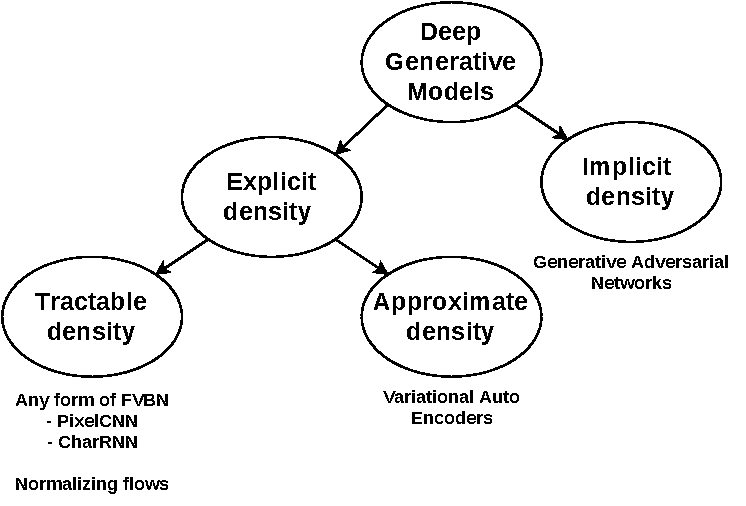
\includegraphics[width=0.85\linewidth]{background/images/generativetaxonomy}
	\caption[Taxonomy of deep generative models]{Taxonomy of the most common deep generative models.}
	\label{fig:generativetaxonomy}
\end{figure}


\subsubsection{Fully Visible Belief Networks}
The \textit{fully visible belief networks} (FVBN) are a family of probabilistic models that use the chain rule of probabilities to model the probability density of the data ($p_\mathrm{model}(x) \approx p_\mathrm{data}(x)$; \citealp{smith2018}). For that, $p_\mathrm{model}(x)$ is decomposed into a set of conditional probabilities $p(x^{(t)}| x^{(1)}, x^{(2)}, \ldots, x^{(t-1)})$ that when multiplied together form  $p_\mathrm{model}(x)$, as shown in equation \ref{eq:fvbn}.

\begin{equation}
	\label{eq:fvbn}
	p_{model}(x) = \prod_{i=1}^{T} p(x^{(t)}| x^{(1)}, x^{(2)}, ..., x^{(t-1)})
\end{equation}

The FVBN models provide a fully tractable probability density function \autocite{Goodfellow2016}, and are well suited for modeling sequential data such as text or speech \autocite{Wang2017,Shen2018,liu2019b}. They have also been applied to model images, by turning them into sequences of pixels \autocite{Oord2016, Oord2016b}.

The basic operation of FVBN is very simple. At training time, a model is trained to predict the next sample of a sequence $x(t)$, given the previous samples $ x^{(1)}, x^{(2)}, ..., x^{(t-1)}$. This operation is known as \textit{teacher forcing} \autocite{williams1989, Goodfellow2016, Goyal2016}, as the model is feed with the original samples of the sequence being modeled. At inference time, a start sample $\hat{x}^{(1)}$ is provided as input for the model to predict a probability distribution $p(x^{(2)}|\hat{x}^{(1)})$ from which the next sample is drawn $\hat{x}^{(2)}$. Subsequently, $ \hat{x}^{(1)}$ and $\hat{x}^{(2)}$ are feed into the model to get the probability distribution of the third sample $p(x^{(3)}|\hat{x}^{(1)}, \hat{x}^{(2)})$, from where $x^{(3)}$ is drawn. The process continues until a stop criterion is reached. The inference operating mechanism is commonly referred \textit{free running mode} \autocite{Goodfellow2016}, as the model is feed with previously generated samples, and does not depend on the ground truth signal. Normally, a deep learning model is used to train FVBN, in particular RNNs and transformers are some of the most common choices. Figure \ref{fig:charrnn} shows an example of \textit{char-rnn} \autocite{Sutskever2011, Graves2013}, a FVBN used to generate natural language. 

\begin{figure}
	\centering
	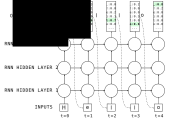
\includegraphics[width=0.8\linewidth]{background/images/char_rnn}
	\caption[\textit{Char-rnn} architecture]{Architecture of \textit{char-rnn}, a deep learning model used for natural language generation at character level, based on a multilayer recurrent neural network. The nodes represent RNN cells (e.g. GRU cells) and the rectangles are the inputs and outputs of the model. The dashed arrows represent the character sampling process.}
	\label{fig:charrnn}
\end{figure}


As it can be noticed, the training process, provided with the right algorithms, can be performed in parallel. However, the inference process needs to be done sequentially, given that to generate future samples, all the past samples need to have been previously generated. For this reason, FVBN are known to be inefficient at inference time when used to generate long sequences.

As an example, a shallow version of the \textit{char-rnn} model of order\footnote{The probability distribution of the next character is conditioned to the previous 100 characters.} 100 has been trained using 800 books from the open source \textit{Gutenberg} project\footnote{https://www.gutenberg.org/} \autocite{gerlach2020}. The model consists of a recurrent neural network that is trained to predict the \textit{Multinoulli} distribution for the next character, conditioned to the previous 100 characters as input. The code of this model can be found in the repository linked in the footnote\footnote{\url{https://github.com/ivallesp/simple_chatbot}}. The following is an example of generation where the first 100 characters of the \textit{War of the Worlds} book from \textit{Herbert George Wells} are fed as input.

\chapquote{\textbf{``No one would have believed in the last years of the nineteenth century that this world was being wat}ched together far out
	to the thought, 'that will cled it announced for them bloody I have
	last instant all the strayes as thomass us? This is, and the single
	War camp, until we proguted it toward the mouncin to lint of the
	enemy respectful, then the ribonament had been their courts and papers
	she been ended bent tense freely after good to the eyes to avole.
	The gather flooded by Wayer a great time home engaged in the
	exhausting day of the dutie of summers and jangers untourant altogether
	of mountains. But was the mystery arising half die for some regarding
	the raider. This top was a Catelumberhand life by the river were
	business, and other ebbsake and septimum at the campaich, wa, and he
	showed my brethren.''}{\textit{char-rnn}}{2017}

It can be noticed that the model has been able to generate many grammatically correct words, although the text generated is not coherent. For that, more sophisticated approaches would be needed. \textit{GPT-3} \autocite{floridi2020} is a modern example of deep language model.

Other example of modern FVBN application is presented in \citet{Oord2016} and \citet{Oord2016b}, an extension of \textit{char-rnn} to two dimensions, where a set of pixels of an image are given as input to the model, and its task is to predict the remaining pixels in an auto-regressive manner. 


\subsubsection{Variational auto-encoders}
\textit{Variational auto-encoders} (VAE hereafter) are another alternative family of methods used to approximate $p_\mathrm{data}(x)$ \autocite{kingma2019}. VAEs are the probabilistic versions of \textit{auto-encoders} (AE). An AE is a deep learning model that is trained to reconstruct its input $\mathbf{x}$ in its output $\mathbf{y}$. The input vector $\mathbf{x}$ is transformed into a compressed representation $\mathbf{h}=f_e(\mathbf{x})$ using an encoder $f_e$, and that vector $\mathbf{h}$ is feed into the decoder $f_d$ to produce $\mathbf{\hat{y}}=f_d(\mathbf{h})=f_d(f_e(\mathbf{x}))$. The representation $\mathbf{h}$ is a vector of lower dimension than $\mathbf{x}$, so the encoder is forced to prioritize which aspects of the input should be included in $\mathbf{h}$ so that the decoder can recover $\mathbf{y}\approx \mathbf{x}$ \autocite{Goodfellow2016} with the minimum error. The encoder and the decoder are generally deep learning models.

The main idea of VAEs consists on replacing the $\mathbf{h}$ vector by the parameters of a distribution ($\mathbf{\upsilon}$), generally chosen to be a \textit{Gaussian} $N(\mu,\sigma)$, from which a latent vector is sampled $\mathbf{z} \sim p(\mathbf{\upsilon})$. Once the model is trained, new samples $\mathbf{\hat{x}}$ can be generated by decoding samples drawn from the prior distribution $\mathbf{\hat{x}} = f_d(\mathbf{z})$ where $\mathbf{z} \sim p(\mathbf{\upsilon})$. The structure of this deep learning architecture is shown in figure \ref{fig:vae}.




VAEs provide an explicit but intractable density function which cannot be directly optimized \autocite{Goodfellow2016}. Instead, variational \textit{Bayesian} methods are used to approximate the intractable probability distributions. In this setting, the posterior probability $p_\mathbf{\theta}(\mathbf{z}|\mathbf{x})$ is intended to be computed. Applying the \textit{Bayes} theorem, we can express $p_\mathbf{\theta}(\mathbf{z}|\mathbf{x}) = \frac{p_\mathbf{\theta}(\mathbf{x}|\mathbf{z}) \cdot p_\mathbf{\theta}(\mathbf{z})}{p_\mathbf{\theta}(\mathbf{x})}$. In this equation, $p_\mathbf{\theta}(\mathbf{x}) = \int{p_\mathbf{\theta}(\mathbf{x}) \cdot p_\mathbf{\theta}(\mathbf{x}|\mathbf{z})} \,d\mathbf{z}$ is intractable, and hence it is not possible to optimize the parameters of a model that approximates that distribution using maximum likelihood. Here is where variational methods take place. 

\begin{figure}[h!]
	\centering
	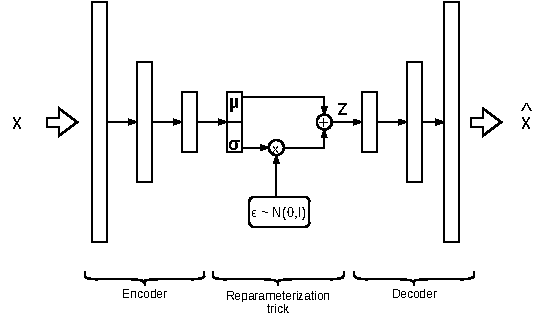
\includegraphics[width=1\linewidth]{background/images/vae}
	\caption[\textit{Variational auto-encoder}]{Diagram showing how a \textit{variational auto-encoder} is structured. }
	\label{fig:vae}
\end{figure}

A known probability distribution $q$ with parameters $\phi$ will be used to approximate $p$ so that $q_\phi(\mathbf{z}|\mathbf{x}) \approx p_\mathbf{\theta}(\mathbf{z}|\mathbf{x})$. With that aim, the \textit{Kullback-Leibler} divergence ($D_{KL}$) metric will be used to minimize the differences between the two distributions, as shown in equation \ref{eq:dklvae} \autocite{kingma2019}. $\mathcal{L}(\mathbf{x}, \mathbf{\theta}, \phi)$, from equation \ref{eq:lbvae}, represents a lower bound (often referred as evidence lower bound, \textit{ELBO}, or negative free energy), given that $D_{K L}\left(q_{\phi}(\mathbf{z} \mid \mathbf{x}), p_{\mathbf{\theta}}(\mathbf{z} \mid \mathbf{x})\right)$ is always greater or equal to zero (see the optimization function in equation \ref{eq:vaelbasloss}). As the lower bound is tractable, the optimization problem can be approximated as shown in equation \ref{eq:vaeopt}. Hence, maximizing the lower bound assures that the log-likelihood is at least as large as its lower bound \autocite{wei2021}.

\begin{equation}
\label{eq:dklvae}
\min_{\phi} D_{KL}\left(q_\phi(\mathbf{z}|\mathbf{x}), p_\mathbf{\theta}(\mathbf{z}|\mathbf{x})\right)
\end{equation}

\begin{equation}
\label{eq:lbvae}
\begin{aligned}
\log \left(p_{\mathbf{\theta}}(\mathbf{x})\right) =& \underbrace{D_{K L}\left(q_{\phi}(\mathbf{z} \mid \mathbf{x}) \| p_{\mathbf{\theta}}(\mathbf{z} \mid \mathbf{x})\right)}_{>0} \ldots \\
&+\underbrace{\mathbb{E}_{\mathbf{z}} \log p_{\mathbf{\theta}}(\mathbf{x} \mid \mathbf{z})-D_{KL}\left(q_{\phi}(\mathbf{z} \mid \mathbf{x}), p_{\mathbf{\theta}}(\mathbf{z})\right)}_{\mathcal{L}(\mathbf{x}, \mathbf{\theta}, \phi)}
\end{aligned}
\end{equation}

\begin{equation}
\label{eq:vaelbasloss}
\log p_{0}(\mathbf{x}) \geq \mathcal{L}_{\mathbf{\theta}, \phi}\left(\mathbf{x}\right)
\end{equation}

\begin{equation}
\label{eq:vaeopt}
\mathbf{\theta}, \phi \leftarrow \underset{\mathbf{\theta}, \phi}{\arg \max } \sum_{i=1}^{N}\left(\mathcal{L}_{\mathbf{\theta}, \phi}(\mathbf{x})\right)
\end{equation}

The first term of the lower bound of equation \ref{eq:lbvae} ($\mathbb{E}_{\mathbf{z}} \log p_{\mathbf{\theta}}(\mathbf{x} \mid \mathbf{z})$) is known as the reconstruction error, and measures how dissimilar the input and the output are. The second term ($D_{K L}\left(q_{\phi}(\mathbf{z} \mid \mathbf{x}) \| p_{\mathbf{\theta}}(\mathbf{z})\right)$), usually referred as the divergence error, measures how dissimilar are the prior and the posterior distributions of the encoder. The probability distributions $p_\mathbf{\theta}$ and $q_\phi$ are two separated deep learning models (with parameter sets $\mathbf{\theta}$ and $\phi$). Normally, the prior distribution over the latent variables $P(\mathbf{z})$ is chosen to be an \textit{isotropic Gaussian} \autocite{wei2021} and in order to ensure that the encoder-decoder architecture is differentiable everywhere, the \textit{re-parameterization trick} is used as a mechanism to replace the classical non-differentiable sampling procedure $\mathbf{z} \sim N(\mathbf{\mu}, \mathbf{\sigma})$ by an equivalent version $\mathbf{z} = \mathbf{\mu} + \epsilon \cdot \mathbf{\sigma}$ where $\epsilon \sim N(0,I)$, in which $z$ is differentiable with respect to $\mathbf{\mu}$ and $\mathbf{\sigma}$ \autocite{kingma2019}.


\subsubsection{Generative adversarial networks}
\textit{Generative adversarial networks} (GAN hereafter) are a type of deep generative models first published in 2014 \autocite{Goodfellow2014}. They consist of a dual deep learning model, where the first component, known as the generator, tries to generate realistic data samples, and the discriminator (the generator's adversary) attempts to determine if a given sample is real or generated. As an analogy, one can think of the generator as playing the role of a counterfeiter, and the discriminator playing the role of a police officer. The role of the counterfeiter is to try to fool the police officer, while the latter will try to catch the counterfeiter. Figure \ref{fig:police_counterfeiter} summarizes this process graphically.

The training process of a GAN is generally a zero-sum game, where the optimization succeeds when the system reaches the \textit{Nash} equilibrium \autocite{nash48}. The goal of the algorithm is to learn to represent an estimated distribution ($p_{\mathrm{model}}$) of a given data distribution ($p_{\mathrm{data}}$). Moreover, GANs are designed to be unbiased \autocite{Goodfellow2016}, in the sense that provided with enough data, a model with enough capacity and the proper learning algorithm, the true probability distribution of the data can be perfectly recovered: $p_{\mathrm{model}} = p_{\mathrm{data}}$. As an important practical aspect of GANs, once the algorithm has converged the generator is able to synthesize samples of $p_\mathrm{model}$, but the learned probability density function (PDF) is implicit. GANs provide no access to the learned PDF.

In the GAN systems, the generator $f_g$ is a deep learning model with parameters $\mathbf{\theta^g}$ that takes a latent vector $\mathbf{z} \sim p(\mathbf{z})$ as input, where $p$ is a prior distribution (usually chosen to be a \textit{Gaussian} distribution), and produces a sample $\hat{\mathbf{x}}=f_g(\mathbf{z})$. The discriminator $f_d$ is another deep learning model with parameters $\mathbf{\theta^d}$ that takes a sample $\mathbf{x}$ as input, and produces a binary output $f_d(\mathbf{x})$ that models the probability of the input sample $\mathbf{x}$ being real or generated \autocite{Goodfellow2014}. In this setting, the GAN objective can be formulated as a \textit{minimax} objective, as shown in equation \ref{eq:ganminimax}. The default loss function (represented as $J$), is defined in equation \ref{eq:ganloss}. Unfortunately, the training objective is non-convex in $\theta^g$ and $\theta^d$, which makes training difficult when using complex neural networks, often leading to underfitted models \autocite{Goodfellow2016b,Goodfellow2016}. In a simpler manner, when one of the two networks becomes too strong, the system diverges. Stabilization of the GANs remains an open problem, although some advances have been recently made \autocite{arjovsky2017, shaobo2017, wang2022}.

\begin{equation}
	\label{eq:ganminimax}
	f_g^*, f_d^* = \arg \min_{\theta_g} \max_{\theta_d} J(f_g, f_d)
\end{equation}

\begin{equation}
	\label{eq:ganloss}
	J(\theta^g, \theta^d) = \mathbb{E}_{\mathbf{x}\sim p_\mathrm{data}} \log (f_d(\mathbf{x})) + \mathbb{E}_{\mathbf{x}\sim p_{model}} \log (1 - f_d(\mathbf{x}))
\end{equation}

The generator and discriminator models must be differentiable everywhere, otherwise the model cannot be trained with backpropagation. As an important detail that can be noticed in equation \ref{eq:ganminimax}, both players have a cost function (equation \ref{eq:ganloss}) that depends on the superset  of parameters $\{\theta^g, \theta^d\}$, but every player can only change its own parameters, and not the adversary's.

\begin{figure}[h!]
	\centering
	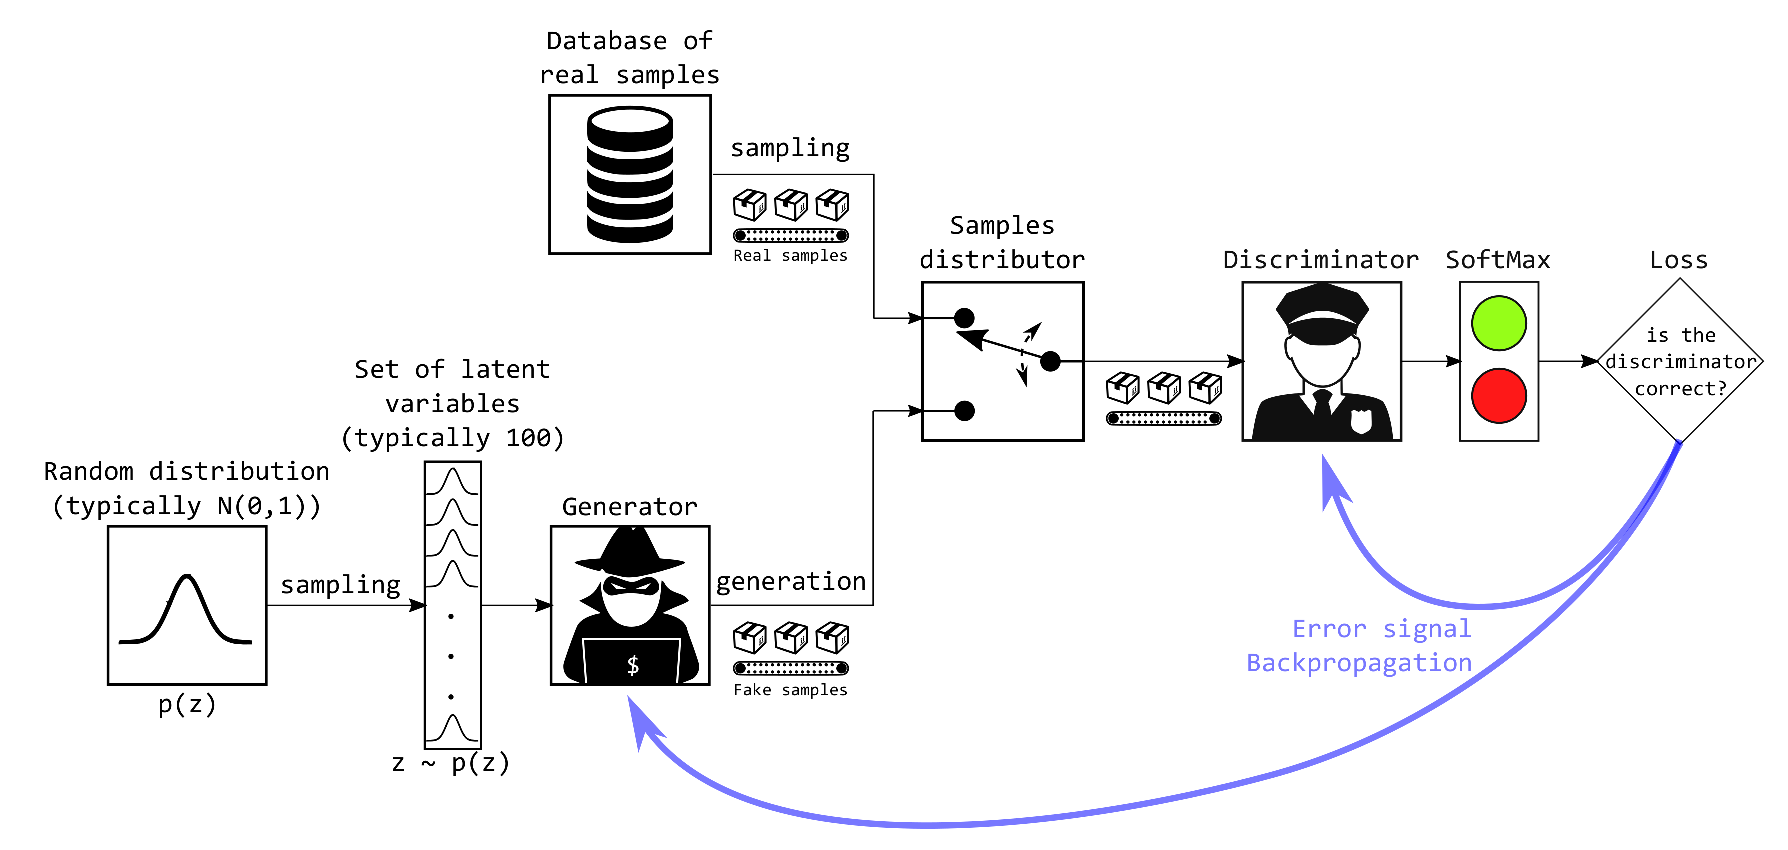
\includegraphics[width=1\textwidth]{background/images/police_counterfeiter.eps}
	\caption[Generative adversarial network]{\textit{Generative adversarial network} diagram, showing the role of the generator and the discriminator and the error signals backpropagated through the network.}
	\label{fig:police_counterfeiter}
\end{figure}

\subsubsection{Normalizing flows} \label{sec:flows}
\textit{Normalizing Flows} are another type of deep generative models that are used to approximate data distributions $p_\mathrm{data}$. These models describe the transformation of a prior density function $p(z)$ into an arbitrarily complex probability distribution $p_\mathrm{model}$, through a series of invertible mappings, by repeatedly applying the rule for change of variables \autocite{rezende2015}. The output of the series of invertible functions applied to the prior distribution is still a valid probability distribution, and hence this type of models is known as normalizing flow.

A flow $f: \mathbb{R}^d \rightarrow \mathbb{R}^d$ is an invertible mapping (i.e. $\exists f^{-1}$) such that $f(f^{-1}(\mathbf{x})) = \mathbf{x}$. The probability density function $p(\mathbf{x})$ could be approximated by applying the rule for change of variables, as shown in equation \ref{eq:flowcov}, where $p(z)$ is known. Notice that the right hand side of the  equation \ref{eq:flowcov} comes from the application of the inverse function theorem \autocite{rezende2015}.

Invertible and differentiable flows are closed under composition \autocite{kobyzev}. This means that when composing multiple flows, the resulting function is still a flow. That property is very important for building deep normalizing flows capable of modeling complex data distributions such as images. It can be easily seen from equation \ref{eq:flowcov}  \autocite{rezende2015} that given a composition of $F$ flows, $\mathbf{x}=f_F \circ ... f_1(\mathbf{z})$, the probability distribution $p_F(\mathbf{z_F})$ can be easily obtained through the application of the change of variables formula, as shown in equation \ref{eq:flowcovcomp} (expressed as log-probability for mathematical convenience), where $h_k$ is the output vector of the flow $f_k$.


\begin{equation}
\label{eq:flowcov}
p_\theta(\mathbf{x}) = p_\theta(f^{-1}(\mathbf{x})) \cdot \left| \det \frac{\partial f^{-1}(\mathbf{x})}{\partial \mathbf{x}} \right| = p(\mathbf{z}) \cdot \left| \det \frac{\partial f(z)}{\partial \mathbf{z}} \right|^{-1}
\end{equation}


\begin{equation}
\label{eq:flowcovcomp}
\log p_\theta(\mathbf{x}) 
= \log p_\theta(\mathbf{z}) + \log  \left| \det \frac{\partial \mathbf{z}}{\partial \mathbf{x}} \right| 
= \log p_\theta(\mathbf{z}) + \sum_{k=1}^{F} \log  \left| \det \frac{\partial \mathbf{h}_k}{\partial \mathbf{h}_{k-1}} \right| 
\end{equation}


The normalizing flow is trained by maximizing the PDF of the samples $\mathbf{x}$, which can be calculated as the probability density of the normalized samples $p(f^{-1}(\mathbf{x}))$ with a volume correction term derived from the change of variables formula, as expressed in \ref{eq:flowcovcomp} \autocite{papamakarios2017}. Once the model is trained, one can sample from the prior distribution $\mathbf{z} \sim p(\mathbf{z})$ and transform that latent variable into a data sample $\hat{\mathbf{x}} = f(\mathbf{z})$ \autocite{rezende2015}.

There are two main restrictions that have to be taken into account when designing neural architectures for normalizing flows. First, each flow block $f_i$ needs to be invertible; and, second, the determinant of the \textit{Jacobian} of each flow block must be fast to compute. These two properties are absolutely necessary for being able to train deep learning based normalizing flows, and they represent the major difficulty currently under research. The most common solution at the time of writing this dissertation is to define the flows $f_i$ as affine-coupling layers \autocite{dinh2018}. Their structure is represented in figure \ref{fig:affinecouplingblock}. More formally, given an input vector $\mathbf{x}$, of size $\mathbf{D}$, an integer $d \in [2,D-1]$, a deep learning model $s$ and another $l$, the affine-coupling layers can be defined as shown in equation \ref{eq:affinecouplingblock}. It can be shown that the determinant of the \textit{Jacobian} of the affine-coupling layer transformation does not depend on the parameters of the networks $l$ and $s$, so they can be as complex as one wants \autocite{dinh2018}. The whole operation can be seen as a scale and shift operation applied over one part of the input vector $\mathbf{x_{d+1:D}}$, and conditioned over the other $\mathbf{x_{1:d}}$. The composition of multiple affine-coupling layers with interleaved shuffling operations builds \textit{RealNVP} \autocite{dinh2018}, a deep normalizing flow that achieved remarkable results in computer vision.

\begin{equation}
\label{eq:affinecouplingblock}
\begin{gathered}
	 \mathbf{y} = \begin{cases} \mathbf{y_{1: d}} & = \mathbf{x_{1: d}} \\
	\mathbf{y_{d+1: D}} & =\mathbf{x_{d+1: D}} \odot s\left(\mathbf{x_{1: d}}\right)+l\left(\mathbf{x_{1: d}}\right)\end{cases} \\
	\mathbf{x} = \begin{cases}
	\mathbf{x_{1: d}} &=\mathbf{y_{1: d}} \\
	\mathbf{x_{d+1: D}} &=\left(\mathbf{y_{d+1: D}}-l\left(\mathbf{y_{1: d}}\right)\right) \odot s\left(\mathbf{y_{1: d}}\right)
	\end{cases}
\end{gathered}
\end{equation}

\begin{figure}[h!]
	\centering
	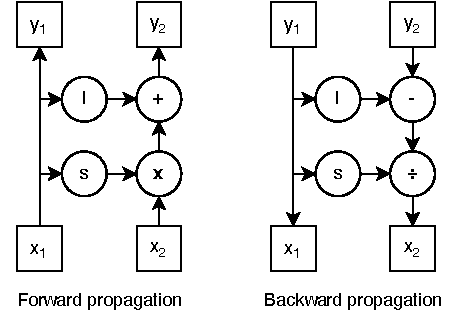
\includegraphics[width=0.5\linewidth]{background/images/affinecouplingblock}
	\caption[Normalizing flows affine coupling layers]{Forward and backward computation graphs for \textit{affine-coupling layers}. Notice that $\mathbf{x_1}$ and $\mathbf{x_2}$ represent the input vector $\mathbf{x}$ split in two parts, and the affine coupling operation produces two vectors $\mathbf{y_1}$ and $\mathbf{y_2}$ of the exact same size as $\mathbf{x_1}$ and $\mathbf{x_2}$, respectively. The nodes with the letters $l$ and $s$ are arbitrarily complex neural networks that, conditioned to the first vector, produce scaling and translation weights to be applied over the second vector.}
	\label{fig:affinecouplingblock}
\end{figure}


Other common solutions to the same problem are known as masked auto-regressive flows \autocite{papamakarios2017}, inverse auto-regressive flows \autocite{kingma2016} or \textit{glow} \autocite{kingma2018}. They will not be covered here because it is out of the scope of this dissertation. More details about \textit{glow} will be given in chapter \ref{ch:tts}.


\subsubsection{Evaluation} \label{sec:dgmevaluation}
One of the most important aspects of any discipline in science is the ability to properly measure the phenomenon under study, and the field of generative models is not an exception. However, measuring how well a generative model performs can be an extremely difficult task \autocite{Goodfellow2016}. There are several approximate approaches that aim to quantify the performance of a generator \autocite{theis2016a}, but we still do not have a general way to tackle this problem.

Many of the applications of generative models deal with multimedia data such as images, music, speech, etc. Our way of determining if a set of synthetic media has good or bad quality is through perceptual judgement. Generative models can be evaluated using perceptual judgement, but as any type of judgement, it may be subject to biases. To avoid a biased evaluation, the evaluation set and the jury needs to be carefully chosen. Even if these pieces are designed carefully, there is still risk that this subjective evaluation completely fails \autocite{Goodfellow2016}. One possible case is the hypothetical example in which a model learns to memorize the training data. In that case, the model will not be succeeding at the generation task, but a perceptual test would score the model with very high performance. Other example could be a model which is collapsed into a mode in the data. For example, given a model that is trained to generate images of cats and dogs, if the model only learns to generate high quality images of cats and never generates dogs, it may get a high score out of a subjective test, while it is completely failing to capture the variability of the data. For these reasons, it is well known that subjective quality of samples is not a reliable way of evaluating generative models \autocite{denton2015}.

Other common way to evaluate generative models consists of measuring the log-likelihood of the $p_\mathrm{model}$ over a test set, in the cases in which the log-likelihood is tractable \autocite{Goodfellow2016}. This approach may be informative in some cases, but it is not a solution at all, as it may often not be correlated with the perceptual quality. One example could be a speech synthesis network that models the silences in the recordings with a very small variance. The probability density in those regions would be extremely high, while perceptually we would not probably be interested on accurately reproducing background noise. Additionally, the comparison of log-likelihoods of different models should be done under the same conditions. Aspects like data processing, the type of algorithm that is used to approximate the log-likelihood or the choice of the prior distribution can bias the results \autocite{Goodfellow2016}.

This topic is still an open research problem, and many studies have already provided some insights about it \autocite{theis2016a, sajjadi2018}. However, the problem remains still unsolved.



